% !tex root = 01.tcp.file.transfer.tex
\documentclass{article}
\usepackage{hyperref}
\usepackage[utf8]{inputenc}
\usepackage{geometry}
 \geometry{
 a4paper,
 total={170mm,257mm},
 left=20mm,
 top=20mm,
 }
 \usepackage{graphicx}
 \usepackage{titling}

 \title{A simple TCP system capable of transfering files
}

\usepackage{listings}
\usepackage{color}

\definecolor{dkgreen}{rgb}{0,0.6,0}
\definecolor{gray}{rgb}{0.5,0.5,0.5}
\definecolor{mauve}{rgb}{0.58,0,0.82}
\definecolor{blue}{rgb}{1,0,0}
\hypersetup{
    colorlinks=true,
    linkcolor=blue,
    filecolor=magenta,      
    urlcolor=cyan,
    pdfpagemode=FullScreen,
    }

\lstset{frame=tb,
  language=Python,
  aboveskip=3mm,
  belowskip=3mm,
  showstringspaces=false,
  columns=flexible,
  basicstyle={\small\ttfamily},
  numbers=none,
  numberstyle=\tiny\color{gray},
  keywordstyle=\color{blue},
  commentstyle=\color{dkgreen},
  stringstyle=\color{mauve},
  breaklines=true,
  breakatwhitespace=true,
  tabsize=3
}

\author{Nguyen Trong Minh}
\date{November 2024}
 
 \usepackage{fancyhdr}
\fancypagestyle{plain}{%  the preset of fancyhdr 
    \fancyhf{} % clear all header and footer fields
    \fancyfoot[R]{
\includegraphics[width=2cm]{usth.png}}
    \fancyfoot[L]{\thedate}
    \fancyhead[L]{Practical 1}
    \fancyhead[R]{\theauthor}
}
\makeatletter
\def\@maketitle{%
  \newpage
  \null
  \vskip 1em%
  \begin{center}%
  \let \footnote \thanks
    {\LARGE \@title \par}%
    \vskip 1em%
    %{\large \@date}%
  \end{center}%
  \par
  \vskip 1em}
\makeatother

\usepackage{lipsum}  
\usepackage{cmbright}

\begin{document}

\maketitle

\noindent\begin{tabular}{@{}ll}
     Developer &  \theauthor \\
     Report writer & \theauthor
\end{tabular}

\section*{System design}
As mentioned in the assignment, we created a system consists of 2 members, a server and a client. 
We also created a file to import constants used in our system.
\begin{lstlisting}
  HOST = '127.0.0.1'
  PORT = 8080
  TOTALCLIENTS = 1
  BUFFERSIZE = 1024
  
  class Signal(Enum):
      CLOSE_SERVER = b'CLS'
      SEND_A_FILE = b'SAF'
      REQUEST_A_FILE = b'RAF'
      SEND_A_REPO = b'SAR'
      REQUEST_A_REPO = b'RAR'
      DONE = b'DON'
      ERROR = b'ERR'
      PING = b'PIN'
      PONG = b'PON'
  
  SIGNALSIZE = getsizeof(Signal.CLOSE_SERVER.value)
\end{lstlisting}
The code above also revealed functions exists in our system that we will go into further detail later.
For the system design, you can see that we created Signal class to store signal used in communication between server and client.
We introduced 5 signals for noticing server about what is going to happen from client side $\texttt{CLOSE\_SERVER, SEND\_A\_FILE, SEND\_A\_REPO, REQUEST\_ A\_FILE, REQUEST\_A\_REPO}$ 
and 4 signals to communicate between server and client $ \texttt{DONE, ERROR, PING, PONG}$. We also fixed size of each bytes buffer to be sent for files' content at 1024 bytes, and for signal is the size of 36 bytes. \\
\\
Our server first bind itself to a port, in our case 127.0.0.1:8080, it then start listening to any connection from client, which is 1 only. 
\begin{lstlisting}
  sock = socket.socket(socket.AF_INET, socket.SOCK_STREAM) 
  sock.bind((HOST, PORT)) 
  sock.listen(TOTALCLIENTS) 

  # Establishing Connections 
  client_socket, clar = sock.accept()
\end{lstlisting}
At this point we used a loop to check if the client has sent any signal to the server to send or request any file. We have 4 functions to send and receive any file as requseted from client.
If the signal sent from client match specific signal addressed for each function, the server executes it. \pagebreak
\begin{lstlisting}
  while True:
    sig = receive_signal(client_socket)
    if sig == Signal.CLOSE_SERVER.value:
        print('closing')
        break
    if sig == Signal.SEND_A_FILE.value:
        receive_file(client_socket, file_name=r'file-transfered/server-receive/recv0.txt')
    if sig == Signal.REQUEST_A_FILE.value:
        file_name = client_socket.recv(BUFFERSIZE)
        send_file(client_socket, file_name.decode())
    if sig == Signal.SEND_A_REPO.value:
        receive_repo(client_socket, r'file-transfered/server-receive/')
    if sig == Signal.REQUEST_A_REPO.value:
        repo_name = client_socket.recv(BUFFERSIZE)
        send_repo(client_socket, repo_name.decode())
    if not sig:
        break
    print(sig.decode())
\end{lstlisting}
With the client, it is simply a sequential code to execute specific task that we defined inside \hyperref[functions]{Function desgin}.
After all, take a look at our server workflow graph:\\
\begin{center}
  \hspace{20pt}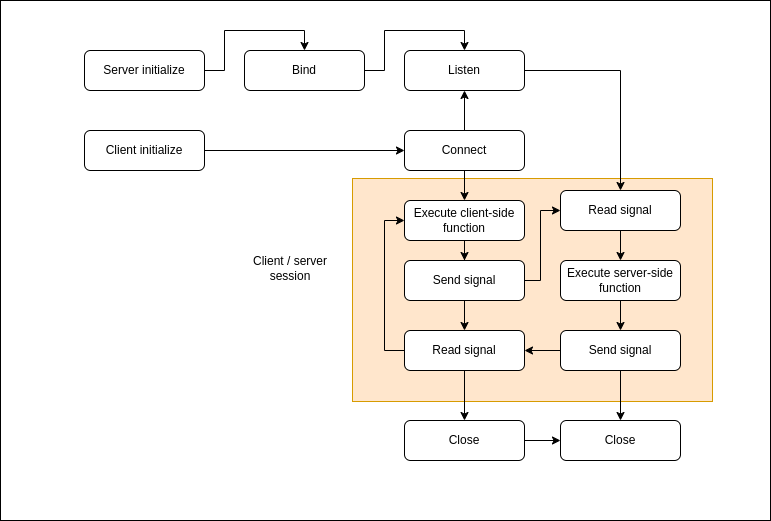
\includegraphics[width=0.9\textwidth]{TCP_server.png} 
\end{center}

\section*{Functions design}\label{functions}
In this section, we will go through 4 functions designed to send 1 or more files between server and client in our system. 
The first funtion is to send a single file from client to server: \pagebreak
\begin{lstlisting}
  def send_file(client_socket : socket.socket, file_name: str):
    """Send a file to server"""
    if not exists(file_name):
        raise FileNotFoundError(f'{file_name} does not exist')
    
    send_signal(client_socket, Signal.SEND_A_FILE )
    sleep(0.1)
    
    client_socket.send(file_name.split("/")[-1].encode())
    sleep(0.1)

    with open(file_name, 'rb') as f:
        while chunk := f.read(BUFFERSIZE):
            client_socket.send(chunk)

    sleep(0.1)
    send_signal(client_socket, Signal.DONE)
\end{lstlisting}

\section*{Other works}
\lipsum[4-4]

\end{document}
